%!TEX root = ../main.tex
\section{Politische Debatte}
  \subsection{Standpunkte einzelner Parteien}
        \begin{frame}<beamer>{Abstimmungsverhalten im Deutschen Bundestag}
\begin{itemize}
        \item Abstimmungsverhalten bei der Einführung der VDS
        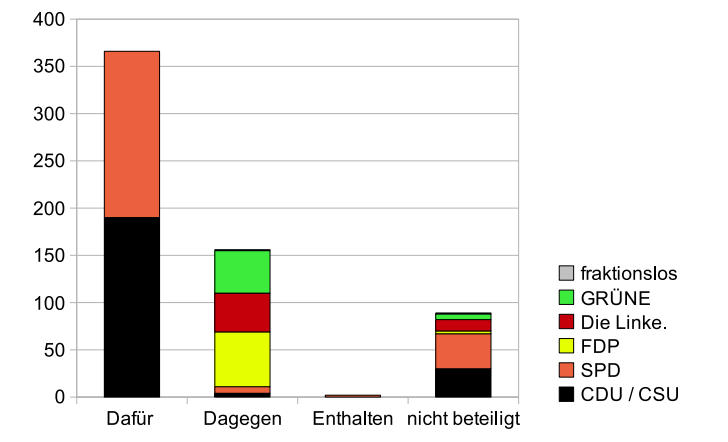
\includegraphics[height=0.9\textheight]{sections/img/abstimmung.png}
    \end{itemize}
    \end{frame}
  
  
    \begin{frame}<beamer>{Standpunkte der CDU}
       \begin{itemize}
        \item setzte sich von Anfang an für VDS ein
        \begin{itemize}
        \item Argumentation: zunehmende Bedrohung durch Terror, Kinderpornographie
         \end{itemize}
        \item 23. April 2014: Das Urteil des Europäischen Gerichtshofs "verdammt uns keineswegs zur Untätigkeit", sagte CDU-Vize Thomas Strobl der "Stuttgarter Zeitung" 
  
      \end{itemize}
    \end{frame}

  \begin{frame}<beamer>{Standpunkte der SPD}
        \begin{quote}
Trotz schwerwiegender politischer und verfassungsrechtlicher
Bedenken werden wir im Ergebnis dem Gesetzentwurf aus
folgenden Erwaegungen zustimmen. Erstens. Grunds¨atzlich
stimmen wir mit dem Ansatz der Bundesregierung und der
Mehrheit unserer Fraktion dahingehend ¨uberein, dass die
insbesondere durch den internationalen Terrorismus und
dessen Folgeerscheinungen entstandene labile Sicherheitslage
auch in Deutschland neue Antworten benoetigt. [. . . ] Eine
Zustimmung ist auch deshalb vertretbar, weil davon
auszugehen ist, dass in absehbarer Zeit eine Entscheidung des
Bundesverfassungsgerichts moeglicherweise verfassungswidrige
Bestandteile fuer unwirksam erklaeren wird.
\end{quote}
    \end{frame}
        
        \begin{frame}<beamer>{Standpunkte der SPD}
        \begin{quote}
Vorratsdatenspeicherung hat mit
Terrorismusbekaempfung relativ wenig zu tun. Ich
waere fuer die Vorratsdatenspeicherung auch dann,
wenn es ¨uberhaupt keinen Terrorismus gabe.
\end{quote}
         \begin{itemize}
   \item Dieter Wiefelsputz, innenpolitischer Sprecher der SPD-Bundestagsfraktion
      \end{itemize}
    \end{frame}
            
    \begin{frame}<beamer>{Standpunkte der SPD}
       \begin{itemize}
        \item 2012 SPD-Mitgliederbegehren zur Abschaffung der VDS gescheitert.
        \item 2013 Koalitionsvertrag fordert Wiedereinführung der VDS
        \item 2014 der Europäische Gerichtshof die EU-Richtlinie zur Vorratsdatenspeicherung für ungültig
         \begin{itemize}
        \item
        SPD-Vize Ralf Stegner: "das Instrument der anlasslosen und flächendeckenden Vorratsdatenspeicherung sei mit dem Urteil "tot"." [Quelle: Stuttgarter Zeitung]
        \item
        baden-württembergische Innenminister Reinhold Gall: der Staat könne auf die Vorratsdatenspeicherung nicht gänzlich verzichten. [Quelle: Deutschlandfunk]
         \end{itemize}
        \end{itemize}

     \end{frame}
     
    \begin{frame}<beamer>{Wortlaut im Koalitionsvertrag 2013}
             \begin{quote}
Wir werden die EU-Richtlinie ueber den Abruf und die Nutzung von Telekommunikationsverbindungsdaten umsetzen. Dadurch vermeiden wir die Verhaengung von Zwangsgeldern durch den EuGH. Dabei soll ein Zugriff auf die gespeicherten Daten nur bei schweren Straftaten und nach Genehmigung durch einen Richter sowie zur Abwehr akuter Gefahren fuer Leib und Leben erfolgen. Die Speicherung der deutschen Telekommunikationsverbindungsdaten, die abgerufen und genutzt werden sollen, haben die Telekommunikationsunternehmen auf Servern in Deutschland vorzunehmen. Auf EU-Ebene werden wir auf eine Verkuerzung der Speicherfrist auf drei Monate hinwirken
\end{quote}
   \end{frame}
     
    \begin{frame}<beamer>{Standpunkte der Grünen/Linken/FDP}
       \begin{itemize}
        \item Die Registrierung der Telekommunikationsdaten stelle alle Bürger unter Generalverdacht
        \item Die Maßnahmen sind ineffizient und unverhältnismäßig
        \item Keine Vereinbarkeit mit Artikel 8 der Europäischen Menschenrechtskonvention
        \item Keine Vereinbarkeit mit dem Grundrecht auf Datenschutz
        \item Unzumutbare Belastungen für die Telekommunikationsindustrie
      \end{itemize}
    \end{frame}
        \begin{frame}<beamer>{FDP Vorschlag: Quick-Freeze}
       \begin{itemize}
        \item Im Verdachtsfall soll die Möglichkeit bestehen anzuordnen die Daten zu speichern
        \item Mithilfe eines zusätzlichen richterlichen Beschluss soll die Möglichkeit bestehen, die Daten abzurufen
      \end{itemize}
    \end{frame}

      \subsection{Protestbewegungen}
    \begin{frame}<beamer>{Protestbewegungen}
       \begin{itemize}
        \item Arbeitskreis Vorratsdatenspeicherung
        \item 11. Oktober 2008: Demonstration "Freiheit statt Angst" mit 15.000 Teilnehmern in Berlin
      \end{itemize}
    \end{frame}
        \begin{frame}<beamer>{Kritik aus dem historischen Kontext}
       \begin{itemize}
        \item totalitäre Überwachung im 3. Reich
        \item Überwachung der Stasi in der DDR
        \item Befürchtung die Ausweitung der Überwachung könnte die Demokratie aushöhlen und letztlich abschaffen.
      \end{itemize}
    \end{frame}
    
          \subsection{Vorratsdatenspeicherung in Österreich}
    \begin{frame}<beamer>{Bilanz der Vorratsdatenspeicherung in Österreich}
        \begin{itemize}
        \item 312 Fälle gab es Auskunft über Vorratsdatenspeicherung
        \item 438 Delikte wurde Vorratsdatenspeicherung abgefragt
        \item 161 erledigten Rechtssachen soll in 71 Fällen die Vorratsdatenspeicherung eine Betrag zur Aufklärung geleistet haben
        \item die meisten Abfragen gab es nicht bei schweren Verbrechen, wie Terrorismus und Mord sondern
        \item die meisten gab es bei Diebstahl(106) und Stalking
        \item Kosten für die Steuerzahler bisher 2,3 Millionen Euro
        \item Man rechnet mit jährliche Gesamtkosten von 8 Millionen Euro.
        \item Stand: 09.07.2013 
         \end{itemize}
    \end{frame}

    
    


